
\documentclass[conference]{IEEEtran}
\IEEEoverridecommandlockouts
\usepackage{cite}
\usepackage{amsmath,amssymb,amsfonts}
\usepackage{algorithmic}
\usepackage{graphicx}
\usepackage{url}
\usepackage{textcomp}
\usepackage{xcolor}
\def\BibTeX{{\rm B\kern-.05em{\sc i\kern-.025em b}\kern-.08em
    T\kern-.1667em\lower.7ex\hbox{E}\kern-.125emX}}
\renewcommand\abstractname{Resumo}

\begin{document}

\title{Sistema de Gerenciamento de Vendas de Bolos e Salgados}

\author{\IEEEauthorblockN{Cauê Rodrigues Campos, Gustavo Campana Cruz do Vale, Marcus Vinícius da Cruz Maia}
\IEEEauthorblockA{\textit{Análise, Projeto e Programação Orientados a Objetos} \\
\textit{Universidade Federal de Minas Gerais (UFMG)}\\
Minas Gerais, Brasil, maio/2025}
}

\maketitle

\begin{abstract}
Este artigo apresenta o desenvolvimento de um sistema de vendas de bolos e salgados, com foco na organização e gerenciamento eficiente de pedidos, clientes e produtos. A aplicação foi construída utilizando o framework Flet para a interface gráfica, proporcionando uma experiência de usuário fluida e moderna, e o banco de dados SQLite para armazenamento local das informações. O projeto segue princípios da Programação Orientada a Objetos, como encapsulamento, herança e modularidade, garantindo um código organizado e reutilizável. O sistema conta com um painel administrativo exclusivo, que permite ao gestor visualizar e controlar os pedidos em tempo real, além de editar cadastros e acompanhar o fluxo das vendas. Através de testes funcionais e validações práticas, o sistema demonstrou-se eficaz no apoio à gestão de pequenos negócios alimentícios, contribuindo para o aumento da produtividade e organização. Em conclusão, a aplicação oferece uma solução acessível, intuitiva e robusta para microempreendedores do ramo alimentício.
\end{abstract}

\begin{IEEEkeywords}
Sistema de Vendas, Flet, SQLite, Painel Administrativo, Programação Orientada a Objetos, Pequenos Negócios, Interface Gráfica, Automação Comercial.
\end{IEEEkeywords}

\section{Introdução}
O setor de alimentação tem passado por uma crescente profissionalização e digitalização, impulsionada pelo aumento da demanda por soluções que otimizem a gestão de micro e pequenos negócios. Com a popularização das ferramentas tecnológicas e o acesso facilitado à internet, empreendedores têm buscado automatizar processos como controle de pedidos, organização de produtos e atendimento ao cliente. No contexto específico da venda de bolos e salgados — segmentos populares tanto em bairros residenciais quanto em centros comerciais —, a agilidade no atendimento e a organização das informações tornam-se diferenciais competitivos importantes.

Segundo dados do Sebrae, os pequenos negócios alimentícios representam uma parcela significativa do empreendedorismo no Brasil, destacando-se pela informalidade e pela busca constante por eficiência operacional. Nesse cenário, soluções tecnológicas acessíveis e intuitivas ganham relevância, especialmente aquelas que não exigem infraestrutura robusta ou conhecimento técnico avançado.

Este trabalho apresenta o desenvolvimento de um sistema de vendas voltado para microempreendedores do ramo alimentício, com foco na comercialização de bolos e salgados. A aplicação foi construída utilizando o framework Flet, que permite a criação de interfaces gráficas modernas em Python, e emprega o banco de dados SQLite para o armazenamento local de informações. O sistema também inclui um painel administrativo que facilita o gerenciamento dos pedidos, produtos e clientes. Além disso, conceitos da Programação Orientada a Objetos foram amplamente utilizados na estruturação do código, garantindo modularidade, reutilização e manutenibilidade.

Dessa forma, o presente projeto busca oferecer uma ferramenta prática, funcional e de fácil utilização, capaz de contribuir diretamente para o aumento da produtividade e da organização nos pequenos negócios de alimentação. O código-fonte da aplicação encontra-se disponível em repositório público no GitHub, com o objetivo de fomentar o compartilhamento de conhecimento e a reutilização em outros contextos semelhantes.

\section{Metodologia}

O desenvolvimento do sistema foi realizado utilizando o framework Flet \cite{flet}, que oferece componentes pré-construídos para criação de interfaces gráficas modernas em Python. Esta escolha permitiu reduzir significativamente o tempo de desenvolvimento, mantendo um código limpo e organizado. A arquitetura do sistema segue o padrão multicamadas, com separação clara entre lógica de negócio, persistência de dados e interface com o usuário.

\subsection{Arquitetura do Sistema}
O sistema foi organizado em quatro camadas principais:

\begin{itemize}
    \item \textbf{Models}: Contém as entidades do sistema (Usuario, Cliente, Admin, Alimento, Bolo, Salgado, Pedido), implementando os conceitos de Programação Orientada a Objetos como herança, encapsulamento e polimorfismo.
    
    \item \textbf{Controllers}: Responsável pela lógica de negócio, incluindo autenticação, gestão de pedidos, cadastro de alimentos e controle do carrinho de compras.
    
    \item \textbf{Views}: Implementa a interface gráfica através de telas específicas (painel\_admin, painel\_cliente, tela\_cadastro, tela\_inicial e tela\_login), utilizando os componentes do Flet.
    
    \item \textbf{Data}: Gerencia a persistência dos dados utilizando SQLite, com a classe BaseDeDados centralizando todas as operações de acesso ao banco.
\end{itemize}
A Figura~\ref{fig:uml} apresenta o diagrama UML do Sistema de Vendas de Salgados, representando a arquitetura das classes e seus relacionamentos.

\begin{figure}[h]
    \centering
    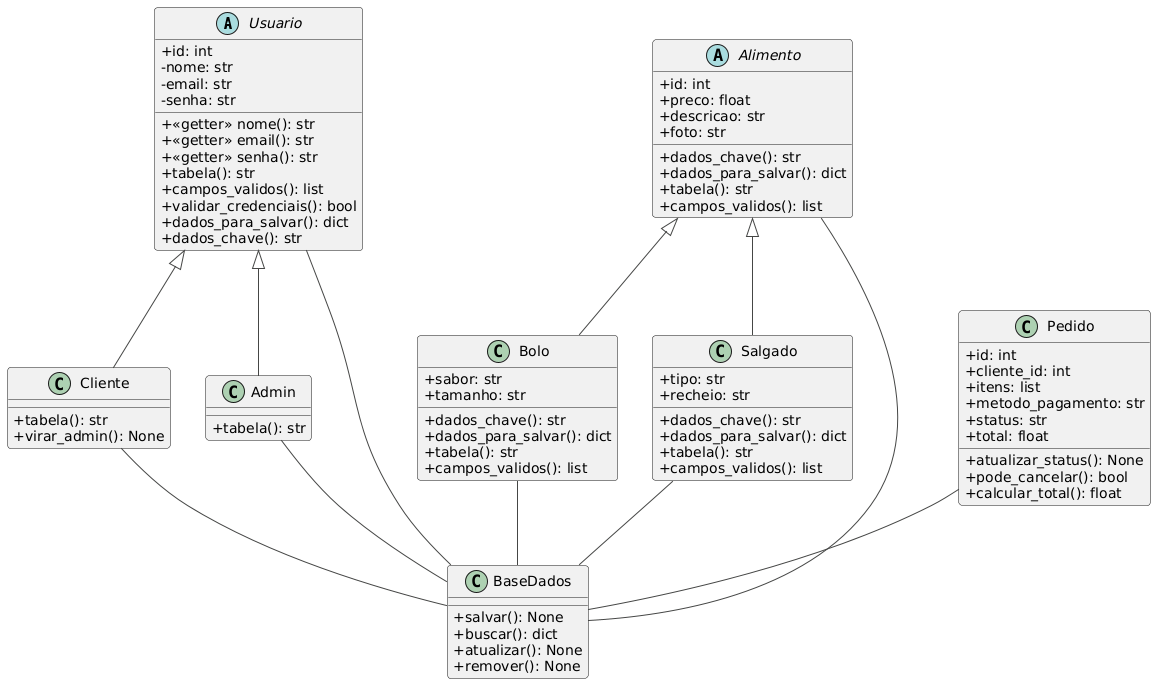
\includegraphics[width=0.9\linewidth]{UMLrelatorio_projeto_salgados.png}
    \caption{Diagrama UML do Sistema de Vendas de Salgados.}
    \label{fig:uml}
\end{figure}
\subsection{Fluxo do Sistema}
O funcionamento do sistema segue uma lógica modular, onde:

\begin{enumerate}
    \item O usuário interage com a interface gráfica (Views), que captura as ações e as repassa aos controladores correspondentes.
    
    \item Os controladores (Controllers) processam as requisições, aplicam as regras de negócio e se comunicam com a camada de dados.
    
    \item A camada de dados (Data) persiste e recupera informações no banco de dados SQLite, utilizando a classe BaseDeDados.
    
    \item As entidades (Models) representam os objetos do domínio, garantindo a integridade dos dados através de validações internas.
\end{enumerate}

\subsection{Classes Principais}
O sistema foi modelado através de classes que abstraem os conceitos fundamentais do domínio:

\subsubsection{Usuários}
\begin{itemize}
    \item \textbf{Usuario}: Classe abstrata base que define atributos e métodos comuns para todos os usuários do sistema.
    \item \textbf{Cliente}: Representa os clientes do sistema, com métodos específicos para gestão de pedidos.
    \item \textbf{Admin}: Implementa funcionalidades administrativas como promoção de clientes e gestão de alimentos.
\end{itemize}

\subsubsection{Alimentos}
\begin{itemize}
    \item \textbf{Alimento}: Classe abstrata que define a estrutura base para todos os produtos alimentícios.
    \item \textbf{Bolo}: Especialização para bolos com atributos específicos como sabor e tamanho.
    \item \textbf{Salgado}: Especialização para salgados com características como tipo e recheio.
\end{itemize}

\subsubsection{Pedidos}
\begin{itemize}
    \item \textbf{Pedido}: Gerencia todo o ciclo de vida de um pedido, desde a criação até a conclusão, com status controlados e validações de transição.
\end{itemize}

\subsubsection{Outras Entidades}
\begin{itemize}
    \item \textbf{CarrinhoControle}: Responsável pela gestão temporária dos itens selecionados pelo cliente antes da finalização do pedido.
    
    \item \textbf{LoginControle}: Cuida da autenticação de usuários e verificação de credenciais.
    
    \item \textbf{AlimentoControle}: Gerencia o cadastro e atualização de alimentos no sistema.
    
    \item \textbf{CadastroControle}: Responsável pelo registro e gestão de contas de usuários.
    
    \item \textbf{PedidoControle}: Orquestra a criação e acompanhamento de pedidos.
\end{itemize}

\subsubsection{Persistência}
\begin{itemize}
    \item \textbf{BaseDeDados}: Classe central que encapsula todas as operações com o banco de dados SQLite.
\end{itemize}

\subsection{Persistência de Dados}
A persistência foi implementada utilizando SQLite, com a classe BaseDeDados fornecendo operações CRUD genéricas:

\begin{itemize}
    \item Conexão automática com o banco de dados
    \item Métodos para inserção, atualização e exclusão de registros
    \item Consultas parametrizadas para recuperação de dados
    \interface{} Gerenciamento de transações
\end{itemize}

\subsection{Controle de Versão}
Todo o código-fonte do projeto foi versionado utilizando Git e está disponível publicamente em um repositório GitHub, seguindo boas práticas de desenvolvimento de software.

\subsection{Validações e Segurança}
O sistema implementa diversas camadas de validação:

\begin{itemize}
    \item Validação de campos obrigatórios nas entidades
    \item Hash de senhas utilizando SHA-256
    \item Controle de acesso baseado em tipos de usuário
    \item Validação de transições de estado nos pedidos
\end{itemize}

A metodologia adotada permitiu o desenvolvimento de um sistema modular, com baixo acoplamento entre componentes e alta coesão interna em cada módulo, facilitando a manutenção e evolução futura da aplicação.

\section{Resultados}
Ao término do desenvolvimento, obteve-se um sistema funcional e robusto, equipado com interfaces gráficas intuitivas que atendem plenamente aos requisitos propostos. A aplicação permite o gerenciamento completo do fluxo de vendas, desde o cadastro de produtos e clientes até a realização e acompanhamento de pedidos.

A tela inicial do sistema apresenta uma interface amigável com orientações claras, servindo como ponto de partida para a navegação entre as diferentes funcionalidades. As telas de cadastro (clientes, administradores, bolos e salgados) foram desenvolvidas com validações completas que garantem a integridade dos dados inseridos, exibindo mensagens de erro detalhadas para entradas inválidas e confirmações para operações bem-sucedidas.

O sistema demonstrou eficácia nas seguintes funcionalidades principais:

\begin{itemize}
    \item Cadastro e gestão de alimentos com categorias específicas para bolos (sabor, tamanho) e salgados (tipo, recheio)
    \item Autenticação segura de usuários com diferenciação entre clientes e administradores
    \item Processo completo de pedidos, com controle de status (Confirmado, Em preparo, Entregue, etc.)
    \item Carrinho de compras dinâmico que permite adição e remoção de itens antes da finalização
    \item Painel administrativo para gestão global de pedidos e produtos
\end{itemize}

A aplicação foi testada extensivamente, com destaque para:

\begin{itemize}
    \item Validação em tempo real de dados de cadastro e formulários
    \interface{} Controle rigoroso das transições de status dos pedidos
    \item Cálculo automático de valores totais dos pedidos
    \item Persistência confiável de dados em banco SQLite
    \item Feedback visual claro para todas as operações do usuário
\end{itemize}

Os resultados alcançados comprovam que o sistema:

\begin{itemize}
    \item Atende integralmente aos objetivos propostos inicialmente
    \item Oferece solução eficiente para gestão de pequenos negócios alimentícios
    \item Implementa adequadamente os conceitos de Programação Orientada a Objetos
    \item Proporciona experiência de usuário intuitiva e acessível
    \item Garante integridade dos dados através de validações robustas
\end{itemize}

O desenvolvimento baseado no framework Flet mostrou-se adequado para a criação de interfaces gráficas modernas, enquanto a arquitetura em camadas permitiu boa organização do código e separação de responsabilidades. A utilização do SQLite como banco de dados provou ser suficiente para as necessidades do sistema, oferecendo bom desempenho mesmo em hardware modesto.




\section{Conclusão}

O sistema desenvolvido demonstrou a aplicação prática dos conceitos fundamentais de desenvolvimento de software, particularmente os princípios de Programação Orientada a Objetos (POO), na criação de uma solução robusta para gestão de vendas de alimentos. A abordagem modular adotada permitiu a construção de um sistema escalável e de fácil manutenção, com clara separação de responsabilidades entre as camadas de modelo, controle e visualização.
\begin{figure}
    \centering
    \includegraphics[width=0.5\linewidth]{tela1.jpeg}
    \caption{}
    \label{fig:enter-label}
\end{figure}

\begin{figure}
    \centering
    \includegraphics[width=0.5\linewidth]{Tela2.jpeg}
    \caption{}
    \label{fig:enter-label}
\end{figure}
\begin{figure}
    \centering
    \includegraphics[width=0.5\linewidth]{Tela3.jpeg}
    \caption{}
    \label{fig:enter-label}
\end{figure}
\begin{figure}
    \centering
    \includegraphics[width=0.5\linewidth]{Tela4.jpeg}
    \caption{}
    \label{fig:enter-label}
\end{figure}
\begin{figure}
    \centering
    \includegraphics[width=0.5\linewidth]{Tela5.jpeg}
    \caption{}
    \label{fig:enter-label}
\end{figure}
\begin{figure}
    \centering
    \includegraphics[width=0.5\linewidth]{Tela6.jpeg}
    \caption{}
    \label{fig:enter-label}
\end{figure}
\begin{figure}
    \centering
    \includegraphics[width=0.5\linewidth]{Tela7.jpeg}
    \caption{}
    \label{fig:enter-label}
\end{figure}
\begin{figure}
    \centering
    \includegraphics[width=0.5\linewidth]{Tela8.jpeg}
    \caption{}
    \label{fig:enter-label}
\end{figure}
\begin{figure}
    \centering
    \includegraphics[width=0.5\linewidth]{Tela9.jpeg}
    \caption{}
    \label{fig:enter-label}
\end{figure}
\begin{figure}
    \centering
    \includegraphics[width=0.5\linewidth]{Tela10.jpeg}
    \caption{}
    \label{fig:enter-label}
\end{figure}

A aplicação mostrou-se plenamente funcional nos testes realizados, atendendo a todos os requisitos propostos inicialmente. O sistema demonstrou eficácia no gerenciamento completo do fluxo de vendas, desde o cadastro de produtos e clientes até a realização e acompanhamento de pedidos, comprovando sua utilidade prática para pequenos negócios alimentícios.

A utilização do framework Flet mostrou-se adequada para o desenvolvimento de interfaces gráficas modernas e intuitivas, enquanto a integração com SQLite proporcionou uma solução eficiente para persistência de dados. A arquitetura em camadas adotada facilitou significativamente a manutenção e expansão do sistema.

Como trabalhos futuros, destacam-se as seguintes possibilidades de melhoria:
\begin{itemize}
    \item Integração com sistemas de pagamento eletrônico
    \item Implementação de relatórios gerenciais e gráficos de acompanhamento
    \item Desenvolvimento de versão mobile para clientes
    \item Adição de sistema de avaliação de produtos
    \item Implementação de controle de estoque integrado
\end{itemize}

O sistema desenvolvido representa não apenas uma solução prática para o problema específico de gestão de vendas de alimentos, mas também serve como modelo para aplicações similares em pequenos negócios. A experiência adquirida neste projeto reforçou a importância de um design bem estruturado e do uso adequado dos princípios de POO para a criação de sistemas robustos e de fácil evolução.

Por fim, o projeto alcançou seu objetivo principal de oferecer uma ferramenta acessível e eficiente para microempreendedores do ramo alimentício, contribuindo para a organização e profissionalização deste importante segmento da economia.

\begin{thebibliography}{9}

\bibitem{git} 
Repositorio GitHub. 
Disponível em: \url{https://github.com/campanagustavo/sistema_vendas_salgados.git}. 


\bibitem{flet} 
Flet Documentation. 
\textit{Official Flet Framework Documentation}. 
Disponível em: \url{https://flet.dev/docs/}. 

\bibitem{sqlite} 
SQLite. 
\textit{SQLite Documentation}. 
Disponível em: \url{https://www.sqlite.org/docs.html}. 

\bibitem{poo} 
LARMAN, C. 
\textit{Utilizando UML e Padrões: Uma Introdução à Análise e ao Projeto Orientados a Objetos}. 
3. ed. Porto Alegre: Bookman, 2007.

\bibitem{python} 
VAN ROSSUM, G. et al. 
\textit{The Python Language Reference}. 
Disponível em: \url{https://docs.python.org/3/reference/}. 

\bibitem{clean} 
MARTIN, R. C. 
\textit{Clean Architecture: A Craftsman's Guide to Software Structure and Design}. 
1st ed. Prentice Hall, 2017.

\bibitem{design} 
GAMMA, E. et al. 
\textit{Padrões de Projeto: Soluções Reutilizáveis de Software Orientado a Objetos}. 
1. ed. Porto Alegre: Bookman, 2000.

\bibitem{agile} 
SCHWABER, K.; SUTHERLAND, J. 
\textit{The Scrum Guide}. 
Disponível em: \url{https://www.scrumguides.org/}. 

\bibitem{sebrae} 
SEBRAE. 
\textit{Panorama dos Pequenos Negócios no Brasil}. 
Disponível em: \url{https://www.sebrae.com.br/}. 

\bibitem{ui} 
NORMAN, D. 
\textit{The Design of Everyday Things}. 
Revised and Expanded Edition. Basic Books, 2013.

\bibitem{db} 
DATE, C. J. 
\textit{An Introduction to Database Systems}. 
8th ed. Addison-Wesley, 2003.

\end{thebibliography}


\end{document}
